\section{Data Interpretation with Graphs}
\textbf{General Equation}

\bigskip
\begin{equationbox}{Graphs}
\textbf{Definition:} A \textbf{\textit{graph}} is a diagram that shows the relationship between two or more variables.
\end{equationbox}

\bigskip
\headertitle{Highest Level of Math by High School Graduates in 2005\footnote{U.S. Department of Education, Institute of Education Sciences, National Center for Education Statistics, High School Transcript Study (HSTS), Mathematics Curriculum Study, 2005.}}
\begin{center}
\begin{tikzpicture}
\pie{5/Algebra I, 16/Geometry, 46/Algebra II, 28/Advanced Math, 5/Calculus}
\end{tikzpicture}
\end{center}

The graph above indicates the highest level of math completed by high school graduates in the U.S. in 2005.

\begin{enumerate}[labelindent=*,style=multiline,leftmargin=*,label=\textbf{Example \arabic*:}]
\item What proportion of students completed Algebra II or Advanced Math over all other courses?
\vfill\item If there are 4200 students in Advanced Algebra, how many students are in Geometry?
\vfill\item If the total number of students represented by the graph is 12,000, how many more students are in geometry than in Algebra I or Calculus?
\end{enumerate}

\vfill
\newpage
\begin{center}
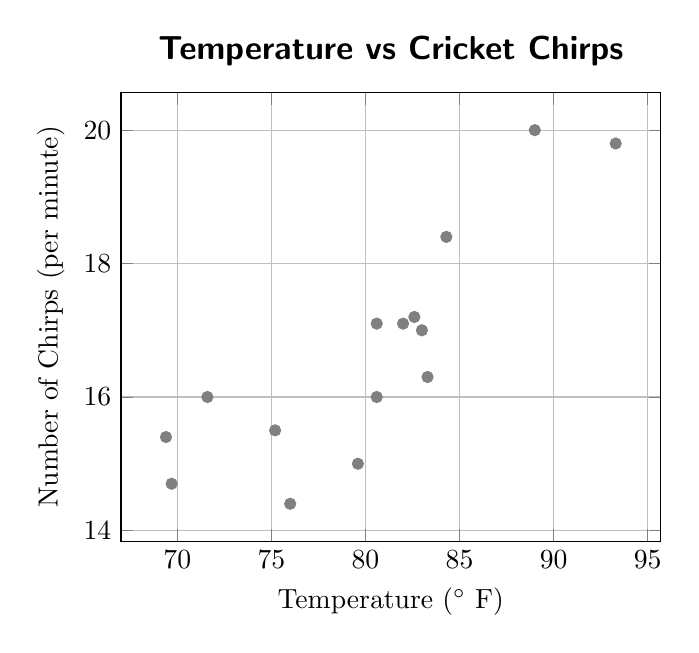
\begin{tikzpicture}
\begin{axis}[
title=\bfseries\fontfamily{cmss}\selectfont{\large Temperature vs Cricket Chirps},
grid=major,
xlabel={Temperature ($^\circ$ F)},
ylabel={Number of Chirps (per minute)},
scatter/classes={a={gray}}]
\addplot[scatter,only marks,scatter src=explicit symbolic]
table[meta=label] {
x y label
89 20 a
71.6 16 a
93.3 19.8 a
84.3 18.4 a
80.6 17.1 a
75.2 15.5 a
69.7 14.7 a
82 17.1 a
69.4 15.4 a
83.3 16.3 a
79.6 15 a
82.6 17.2 a
80.6 16 a
83 17 a
76 14.4 a
    };
\end{axis}
\end{tikzpicture}
\end{center}

The graph above shows the number of chirps a cricket makes per minute versus the temperature of its habitat in degrees Fahrenheit.

\begin{multicols*}{2}
\begin{outline}[enumerate]
\medium

\1 How many points recorded less than 16 chirps for temperatures less than $75^\circ$ F?

\bigskip
\textbf{Equation/Strategy:} \hrulefill

\bigskip
\textbf{Solve:}

\vfill
\2 0
\2 1
\2 2
\2 3
\2 4
\vfill\phantom{}

\columnbreak
\1 Which of the following is likely not a point on the graph?

\bigskip
\textbf{Equation/Strategy:} \hrulefill

\bigskip
\textbf{Solve:}

\vfill
\2 $(60,14)$
\2 $(70,14)$
\2 $(80,18)$
\2 $(90,18)$
\2 $(100,20)$

\vfill\phantom{}
\pagebreak
\advanced

\1 What is the difference in temperature between the temperatures of the highest and lowest number of chirps per minute recorded?

\bigskip
\textbf{Equation/Strategy:}

\bigskip
\textbf{Solve:}

\vfill
\2 5
\2 5.5
\2 6
\2 13
\2 15

\midline

\1 Of the 15 points recorded in this dataset, what proportion of the points are represented by a rate of $5^\circ$ F per chirp or greater?

\bigskip
\textbf{Equation/Strategy:} \hrulefill

\bigskip
\textbf{Solve:}

\vfill
\2 1/15
\2 2/15
\2 1/5
\2 4/15
\2 1/3
\end{outline}
\end{multicols*}